% \begin{blocksection}

\question
Draw the tree that is created by the following statement:

\begin{lstlisting}
Tree(4,
    [Tree(5, []),
     Tree(2,
        [Tree(2, []),
         Tree(1, [])]),
     Tree(1, []),
     Tree(9, []),
     Tree(8,
        [Tree(4, [Tree(6, [])])])])
\end{lstlisting}
\begin{solution}
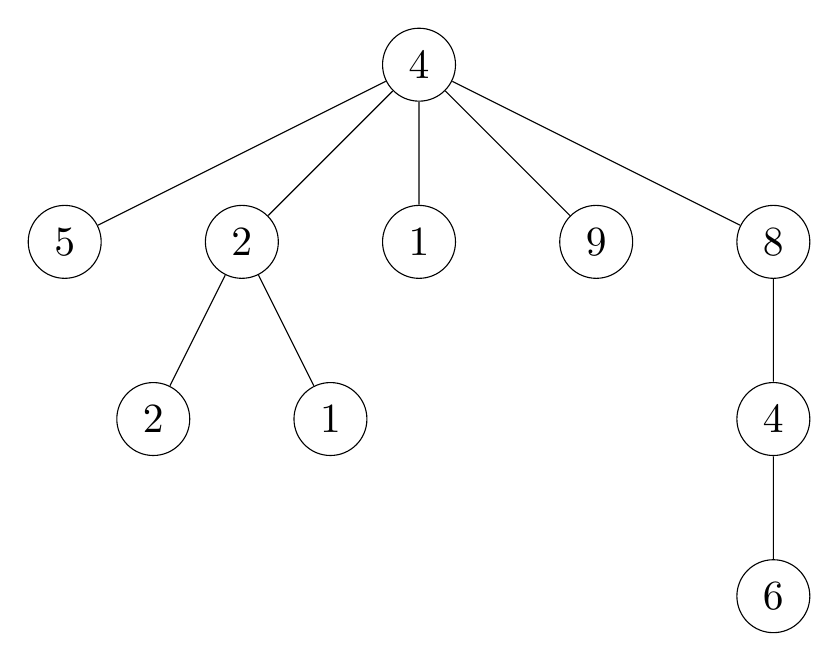
\begin{tikzpicture}[scale=1.5, transform shape]
    \node [circle, draw] (z){$4$}
        child {node [circle, draw] (a) {$5$}}
        child {node [circle, draw] (b) {$2$}
            child {node [circle, draw] (f) {$2$}}
            child {node [circle, draw] (g) {$1$}}
        }
        child {node [circle, draw] (c) {$1$}}
        child {node [circle, draw] (d) {$9$}}
        child {node [circle, draw] (e) {$8$}
            child {node [circle, draw] (h) {$4$}
              child {node [circle, draw] (i) {$6$}}
        }};
\end{tikzpicture}
\end{solution}

% \end{blocksection}
